\documentclass[12pt, a4paper, ngerman]{article}

% Metadata Setup
\newcommand{\Autor}{Leon Kampwerth}
\newcommand{\Was}{Hausarbeit Digitale Bildverarbeitung}
\newcommand{\Kurs}{TINF20IN}
\newcommand{\MatrikelNummer}{5722356}
\newcommand{\Studiengang}{Digitale Bildverarbeitung}

\title{Perceptually Uniform Color Spaces und der Oklab Farbraum}
\author{\Autor}
\date{22.03.2023}

% SETUP
\usepackage{biblatex} % für bibliografie
\usepackage{hyperref} % für links zum klicken
\usepackage{color}    % für Farben (benötigt für listings)
\usepackage{listings} % code schnipsel
\usepackage[ngerman]{babel} % lokalisierung der Titel (Inhaltsverzeichniss)
\usepackage{bookmark} % bookmarks für das PDF
\usepackage{csquotes} % korrekte quotes
\usepackage[version=3]{acro} % akronyme
\usepackage{geometry} % seitengeometrie (margin etc einstellen)
\usepackage{parskip}  % zeilenabstand bei neuem paragraph statt indentierung
\usepackage{fancyhdr} % header und footer
\usepackage{array}    % für bessere Tabellen
\usepackage{titlesec} % um die Titel anzupassen
\usepackage{plantuml} % PLANTUML_JAR has to be set and --shell-escape
\usepackage{amsfonts} % für \mathbb
\usepackage{placeins} % für \FloatBarrier
\usepackage{nicematrix}
 
\hypersetup{
  pdfauthor={\Autor},
  pdftitle={\Was},
  hidelinks
}

\geometry{
  a4paper,
  left=25mm,
  right=25mm,
  headheight=125mm,
  top=35mm,
  bottom=30mm,
  footskip=15mm
}

% title setup 
% make paragraph have a newline
\titleformat{\paragraph}
{\normalfont\normalsize\bfseries}{\theparagraph}{1em}{}
\titlespacing*{\paragraph}
{0pt}{3.25ex plus 1ex minus .2ex}{1.5ex plus .2ex}

% add bibliography
\addbibresource{bibliography.bib}

% header and footer setup
\pagestyle{fancy}
\fancyhf{}
\rhead{\Was}
\lhead{\leftmark}
\lfoot{Autor: \Autor, Kurs: \Kurs}
\rfoot{Seite \thepage}
\renewcommand{\headrulewidth}{1pt}
\renewcommand{\footrulewidth}{1pt}
\fancypagestyle{simple}{
  \fancyhf{}
  \rhead{\Was}
  \lfoot{Autor: \Autor, Kurs: \Kurs}
  \rfoot{Seite \thepage}
}

% acronyms
\acsetup{
  list/display = used,
  pages/display = first
}

%Offizele Akronyme

\newcommand{\reals}{\ensuremath{\mathbb{R}}}
\newcommand{\natnums}{\ensuremath{\mathbb{N}}}

% code snippet setup
\renewcommand{\lstlistingname}{Code-Auszug}
\renewcommand{\lstlistlistingname}{Liste der Code-Auszüge}

\definecolor{black}{rgb}{0,0,0}
\definecolor{green}{rgb}{0,0.5,0}
\definecolor{orange}{rgb}{1,0.45,0.13}		
\definecolor{brown}{rgb}{0.69,0.31,0.31}

% python
\lstdefinelanguage{Python}{
  morekeywords={import, def, from, for, in, if, else, return, True, False, catch, return, null, switch, if, in, while, do, else, case, break},
  morecomment=[l]\#,
  morestring=[b]",
  morestring=[b]""",
  morestring=[b]'
}

\lstdefinestyle{light}{
  % General design
  basicstyle={\footnotesize\ttfamily},   
  frame=b,
  % line-numbers
  xleftmargin={0.75cm},
  numbers=left,
  stepnumber=1,
  firstnumber=1,
  numberfirstline=true,	
  % Quellcode design
  identifierstyle=\color{black},
  keywordstyle=\color{blue}\bfseries,
  ndkeywordstyle=\color{green}\bfseries,
  stringstyle=\color{orange}\ttfamily,
  commentstyle=\color{brown}\ttfamily,
  % Quellcode
  alsodigit={.:;},
  tabsize=2,
  showtabs=false,
  showspaces=false,
  showstringspaces=false,
  extendedchars=true,
  breaklines=true,
}

\begin{document}
\raggedright % sorgt dafür das alles strikt links ausgerichtet wird (und sorgt für mehr seiten)


% Titlepage
\makeatletter
\begin{titlepage}
  \begin{center}
    \vspace*{1cm}
    {\Huge\scshape \Was}\\[2cm]
    \begin{center}
      \linespread{1}\Huge \@title\\[2cm]
    \end{center}
    {\large \Studiengang}\\
    {\large Duale Hochschule Baden-Württemberg\\ Stuttgart}\\[2cm]
    {\large von}\\
    {\large\bfseries \@author}
    \vfill
  \end{center}
  \begin{tabular}{l@{\hspace{2cm}}l}
    Matrikelnummer: & \MatrikelNummer \\
    Abgabedatum:    & \@date          \\
  \end{tabular}
\end{titlepage}
\makeatother

% Table of content
\tableofcontents
\newpage

\thispagestyle{simple}
\printacronyms[name=Abkürzungsverzeichnis, heading=section*]
\newpage

%%%%%%
% Content here
%%%%%% 

\renewcommand{\abstractname}{Abstract} % dass Abstract auch Abstract heißt und nicht zusammenfassung
\begin{abstract}
Dies ist ein Beispiel für ein Abstract \cite{Mustermann:2023}.
\end{abstract}

\section{Farben und Farbräume}
Was ist Farbe? Das ist eine Frage die sehr einfach zu Beantworten scheint, da fast jeder Farben sehen kann. 
Die Encyclopedia Britannica definiert Farbe sinngemäß als Eigenschaft eines Objektes, die durch dessen Farbton, 
Helligkeit und Sättigung beschrieben werden kann. In der Physik werden Farben mit Elektromagnetischer Strahlung in einem
bestimmten Bereich des elektromagnetischen Spektrums beschrieben, der für das menschliche Auge sichtbar ist~\cite{Nassau_2023}.
Gerade hier liegt ein Problem vor, da Farben sowohl Phasikalisch erklärt werden können, 
aber auch Teil der Menschlichen wahrnehmeung sind.

\paragraph{Farbwahrnehmung durch das menschliche Auge}
Die Farbwahrnehmung des Menschen besteht aus mehreren Schritten, 
welche von dem Einfallen der Lichtstrahlen in das Auge bis zur Interpretation der Farbe durch das Gehirn reichen.
Im Auge fällt das Licht auf die Netzhaut, wo sich Zapfen- und Stäbchenzellen befinden, 
welche Photorezeptoren sind, die das Licht in Signale für das Hirn umwandeln.
Für die Farbwahrnehmung sind die Zapfen zuständig, von denen es drei Arten gibt, welche auf unterschieliche Wellenlängen reagieren.
S-Zapfen reagieren auf Wellenlängen im blauen Bereich des sichtbaren Spetrums (ca. 420nm), 
M-Zapfen auf Wellenlängen im grünen Bereich (ca. 530nm) und L-Zapfen auf Wellenlängen im gelb-grünen Bereich (ca. 560nm).
Auch wenn der L-Zapfen auf Licht im gelb-grünen Bereich am stärksten reagiert, 
ist er am wichtigsten für die Wahrnehmung von Rot und wird daher auch als Rotrezeptor bezeichnet~\cite{Zapfen_Auge_2023}.
Die Farbwahrnehmung des Menschen entsteht durch das zusammenspiel der drei Zapfen, 
die, wie in Grafik~\ref{fig:LMS} zu erkennen, durch die Wellenlängen unterschiedlich stark angeregt werden. 

\begin{figure}
  \centering
  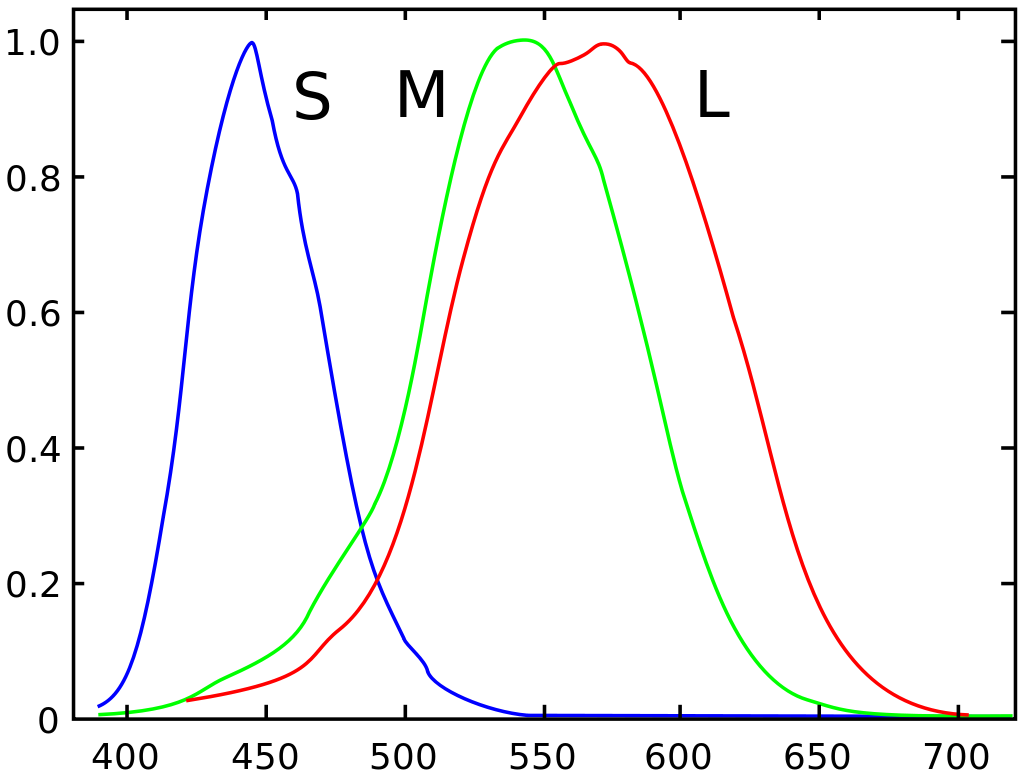
\includegraphics[width=0.5\textwidth]{Grafiken/LMS.png}
  \caption{Normalisierte Empfindlichkeitsspektren menschlicher Zapfenzellen. X Achse: Wellenlänge in nm, Y Achse: Empfindlichkeit, anteilig. Quelle: \cite{LMS_color_space_2023}}
  \label{fig:LMS}
\end{figure}

\paragraph{Farbinterpretation durch das Gehirn}
Die Signale der Zapfen werden im Hirn verarbeitet und interpretiert. 
Dabei werden die Farben durch den Mensch in Form unterschiedlicher Farbeigenschaften wahrgenommen.
Zu diesen Farbeigenschaften zählen der Farbton, die Leuchtkraft, die Helligkeit, das Chroma und die Sättigung.
Die Bedeutung dieser Begriffe wird im später Verlaufe des Artikels noch näher beleuchtet.
Wichtig ist hier, dass die Wahrnehmung dieser Eigenschaften durch viele psychologische Phenomene beeinflusst wird.
Die chromatische Anpassung beschreibt zum Beispiel die Fähigkeit der menschlichen Farbwahrnehmung, 
bei der Betrachtung eines reflektierenden Objekts vom Weißpunkt der beleuchtenden Lichtquelle zu abstrahieren. 
Für das menschliche Auge sieht ein weißes Blatt Papier weiß aus, egal ob die Beleuchtung bläulich oder gelblich ist.
Weitere solcher effekte sind der Bezold-Brücke Effekt und der Abney Effekt, welche sich auf die wahrnehmeung des Farbtons auswirken,
der Stevens Effekt, welcher sich auf den Kontrast auswirkt und der Helmholtz-Kohlrausch Effekt, der sich auf die Leuchtkraft auswirkt.
All diese Effekte sorgen dafür das die Farbwahrnehmung des Menschen schwer zu beschreiben ist und Modelle, die dies Versuchen sehr komplex werden können~\cite{Color_appearance_model_2023}.

\subsection{Farbräume}
Ein Farbsystem stellt das Grundprinzip einer Farbmischung dar, 
beispielsweise durch das Mischen der Lichtfarben Rot, Grün und Blau oder durch das Mischen von Farbpigmenten.
Farbmodelle werden aus einem solchen Farbsystem abgeleitet und ordnen Farben einen eindeutigen Wert (Farborte) zu.
Farbmodelle sind häufig dreidimensional, damit sie einfach visualisiert werden können.
Ein Farbraum wiederum beschreibt alle Farben eines Farbmodells, die durch farbgebende Methoden tatsächlich ausgegeben werden können~\cite{Farbraum_2023}.
Ein Beispiel ist der sRGB Farbraum, welcher ursprünglich für CRTs entwickelt wurde, aber auch heute noch von vielen Displays verwendet wird~\cite{sRGB-Farbraum_2019}.
Die darstellbaren Farben bilden innerhalb des Farbmodells einen Körper, der als Gamut bezeichnet wird.

\subsection{Farbeigenschaften} 
Abgesehen von den von RGB bekannten Farbdimensionen, welche den Anteil der Grundfarben Rot, Grün und Blau beschreiben, 
gibt es noch weitere mögliche Farbdimensionen. Diese Dimensionen nehmen Bezug auf die Farbeigenschaften, nach denen die Farben beschrieben werden können.
Diese Farbeigenschaften stehen im Bezug zueinander und beeinflussen sich teilweise gegenseitig~\ref{fig:ExColordimension}.

\paragraph{Farbton}
Der Farbton (eng. hue) ist eine Eigenschaft der visuellen Wahrnehmung, in welcher eine Fläche 
ähnlich zu einer der Farben rot, gelb, grün oder blau erscheint oder eine Kombination von 
aneinanderliegenden Paaren dieser Farben in einem geschlossenen Farbring ähnelt (vgl. Grafik \ref{fig:Hue})~\cite{Darktable_2023}. 

\begin{figure}
  \centering
  
\includegraphics[width=0.5\textwidth]{Grafiken/Farbring.png}
  \caption{Beispiel eines Farbrings. Quelle: \cite{Hue_2023}}
  \label{fig:Hue}
\end{figure}

\paragraph{Leuchtkraft (und Brillanz)}
Leuchtkraft (eng. brightness) ist eine Eigenschaft der visuellen Wahrnehmung, 
nach der eine Fläche mehr oder weniger Licht zu emmitieren oder zu reflektieren scheint. 
Die Brillanz (eng. brilliance) ist die Leuchtkraft einer Fläche relativ betrachtet zu ihrer Umgebung.
Leuchtkraft ist ein absoluter Wert, während Brillanz in Relation zur Umgebung steht.
Da bei der Bildverarbeitung eine Erhöhung der Leuchtkraft auch die Brillanz erhöht, 
werden diese Begriffe häufig synonym verwendet~\cite{Darktable_2023}.

\paragraph{Helligkeit}
Die Helligkeit (eng. lightness) einer Fläche beschreibt die Leuchtkraft der Fläche 
relativ zu einer ähnlich beleuteten weißen oder stark reflektierenden Fläche~\cite{Darktable_2023}.

\paragraph{Chroma (Buntheit)}
Chroma beschreibt die Farbigkeit einer Fläche, beurteilt im verhältnis zur Leuchtkraft 
einer ähnlich beleuchteten grauen oder weißen Fläche~\cite{Darktable_2023}. 

\paragraph{Sättigung}
Die Sättigung (eng. saturation) ist die Farbigkeit einer Fläche im verhältnis zu ihrer Leuchtkraft~\cite{Darktable_2023}.

\begin{figure}
  \centering
  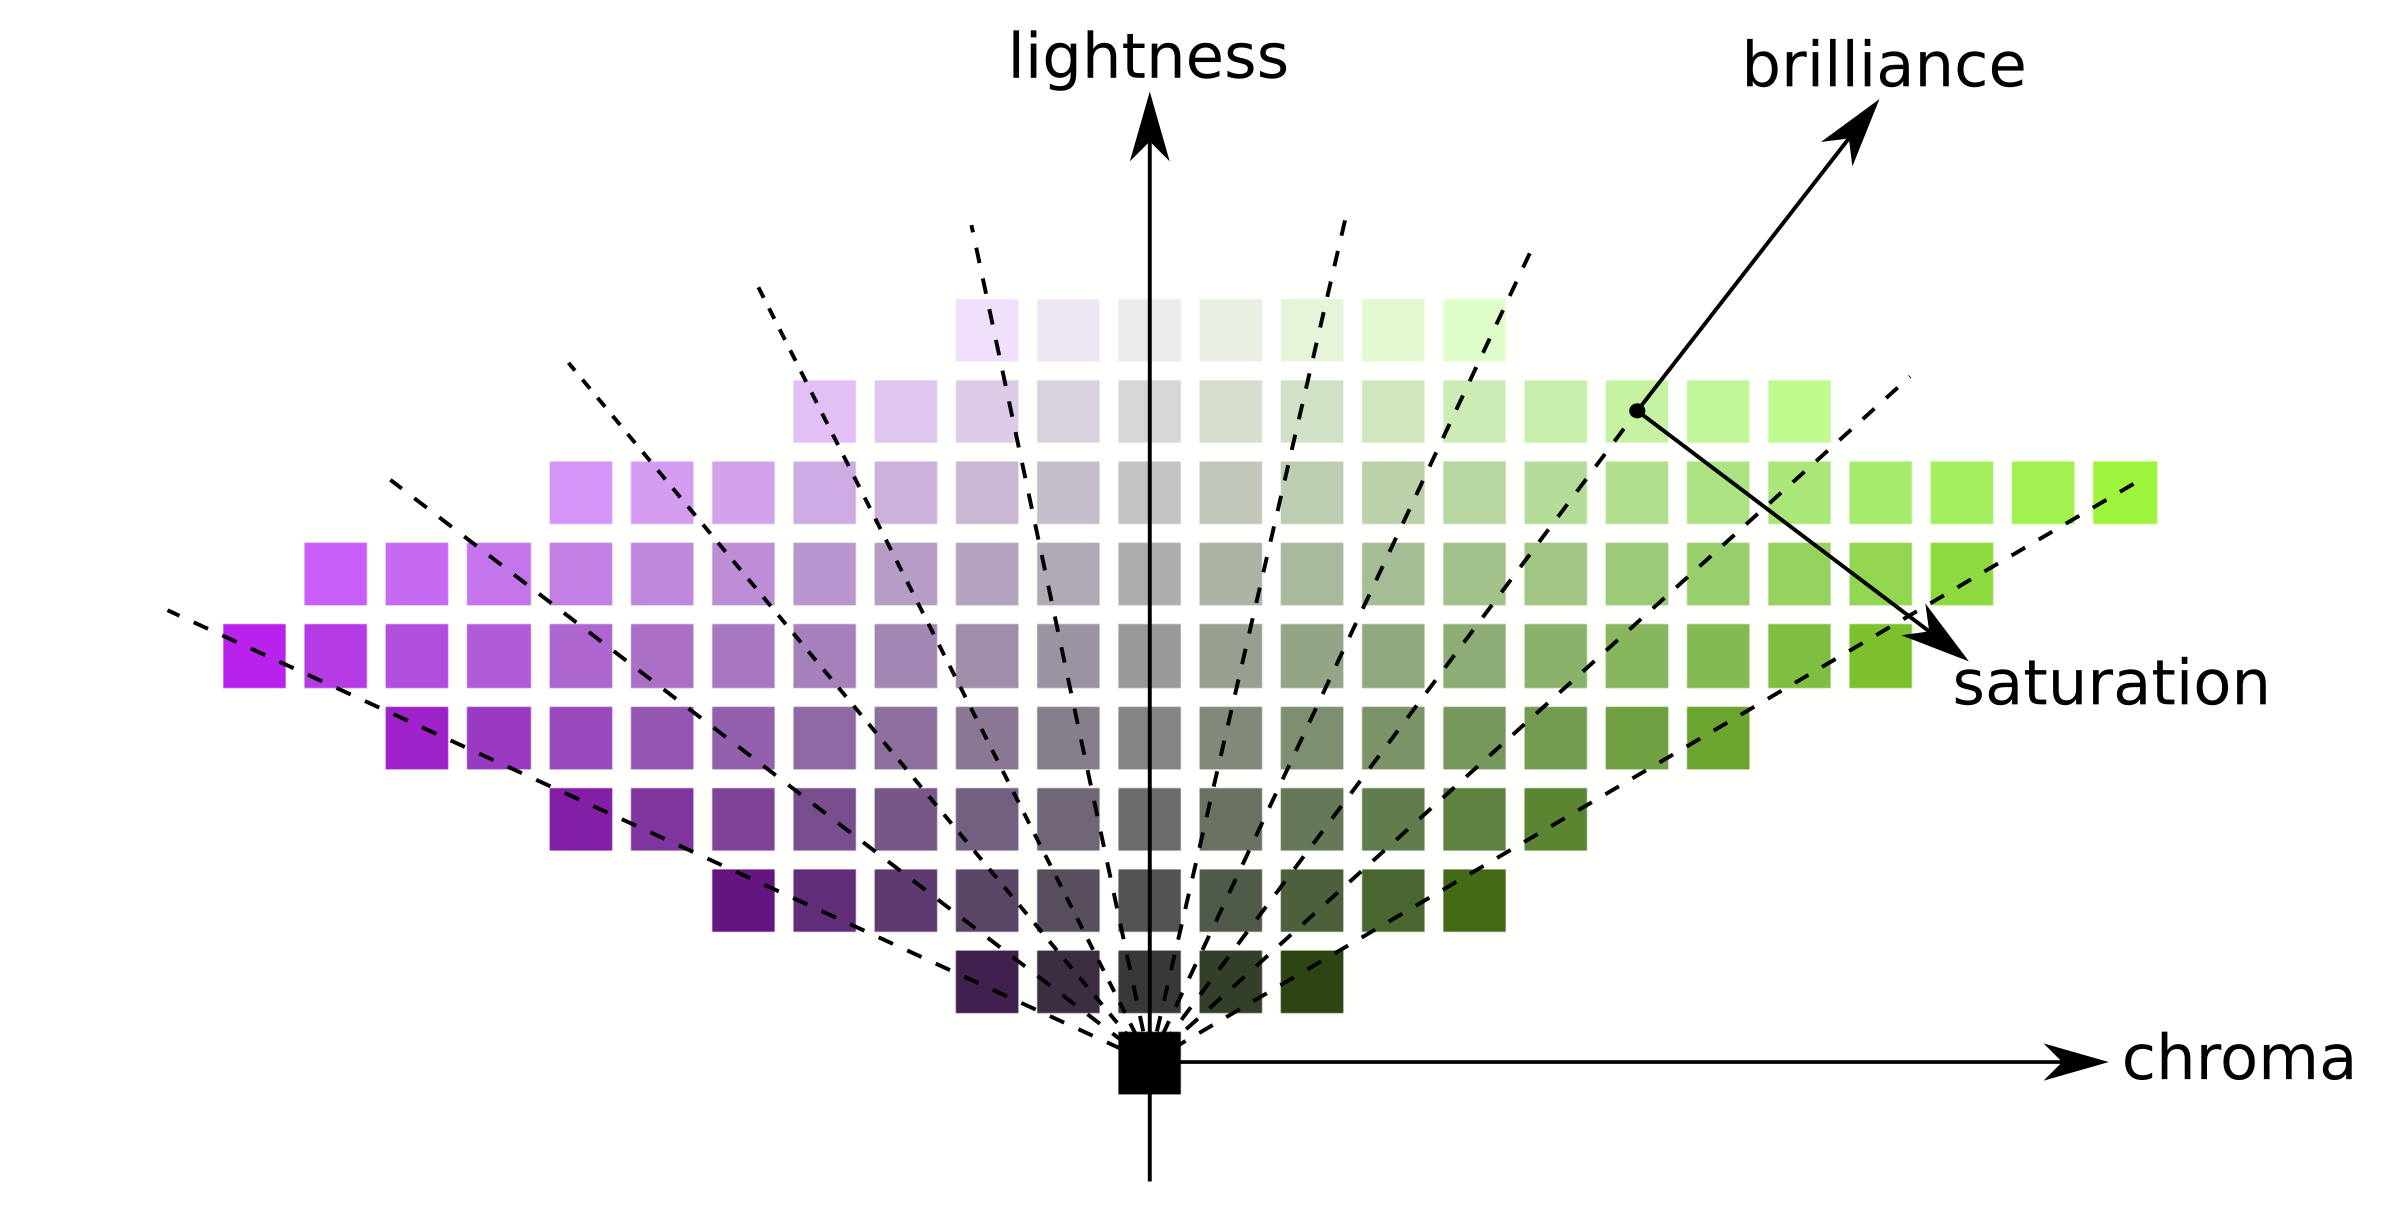
\includegraphics[width=\textwidth]{Grafiken/KoordinatenFarbeigenschaften.png}
  \caption{Beispiel für den Zusammenhang zwischen den Farbeigenschaften. Quelle: \cite{Darktable_2023}}
  \label{fig:ExColordimension}
\end{figure}

\subsection{Unterschieliche Farbräume}
Farben können in vielen unterschiedlichen Farbräumen dargestellt werden. 
Dabei braucht jede Farbe unabhängig vom Farbraum mindestens drei Werte, um beschrieben werden zu können.
Zum einen eine Metrik für Helligkeit oder Leuchtkraft und zum anderen zwei Metriken für die Chromazität 
(nicht zu verwechseln mit Chroma). 
Diese zwei Metriken können zum Beispiel Farbton und Buntheit/Chroma oder komplementäre Farbkoordinaten sein~\cite{Darktable_2023}.
Im Folgenden werden einige Farbräume kurz vorgestellt. Diese Farbräume werden im weiteren Verlauf des Artikels nochmal aufgegriffen.

\paragraph{HSV und HSL}
HSV steht für Hue, Saturation und Value und HSL für Hue, Saturation und Lightness.
Beide Farbräume sind alternative Darstellungen des RGB Farbraums. 
HSL und HSV können beide zylindrische Farbkörper (Abbildung \ref{fig:HSV_HSL}) dargestellt werden, 
wobei hue den Winkel und Saturation den Radius definieren.
Die Höhe des Zylinders ist der Wert, der die Helligkeit als Lightness oder Value beschreibt.
HSV oder HSL werden in Endnutzeranwendungen häufig für Color Picker verwendet ~\cite{HSL_and_HSV_2023}.

\begin{figure}
  \centering
  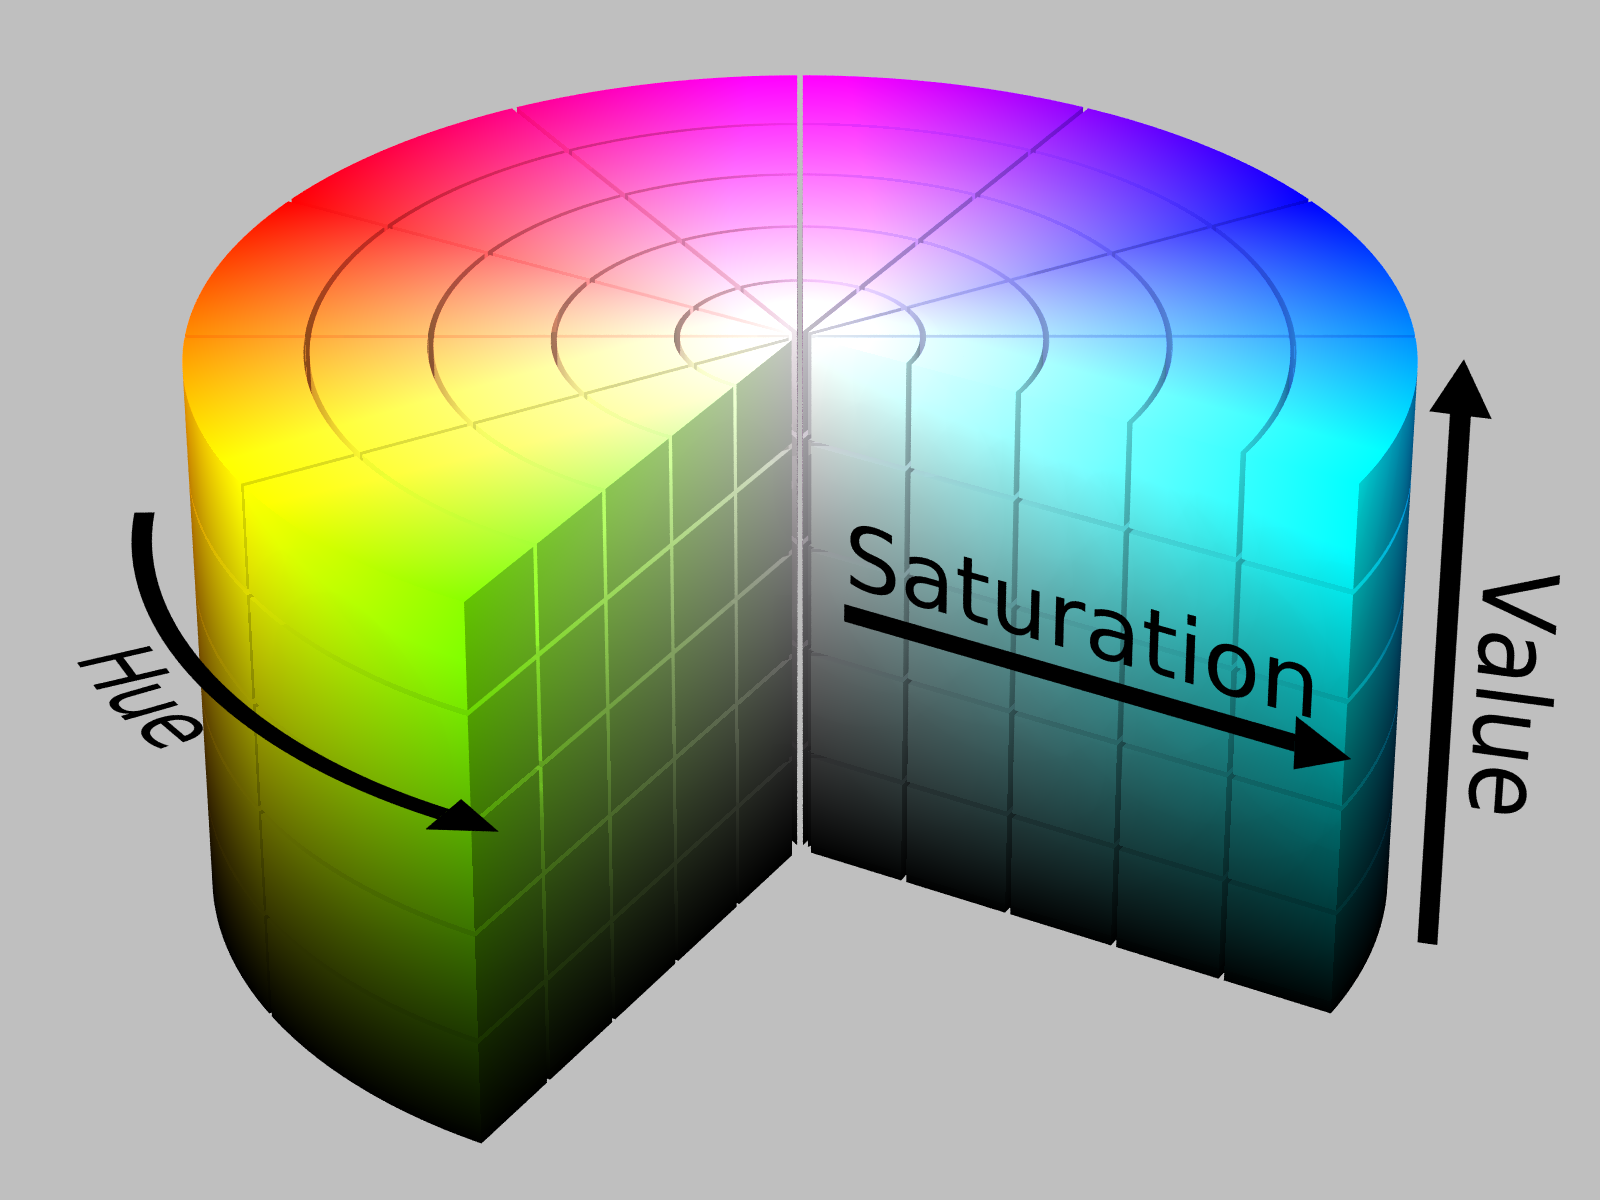
\includegraphics[width=0.48\textwidth]{Grafiken/HSV_Zylinder.png}
  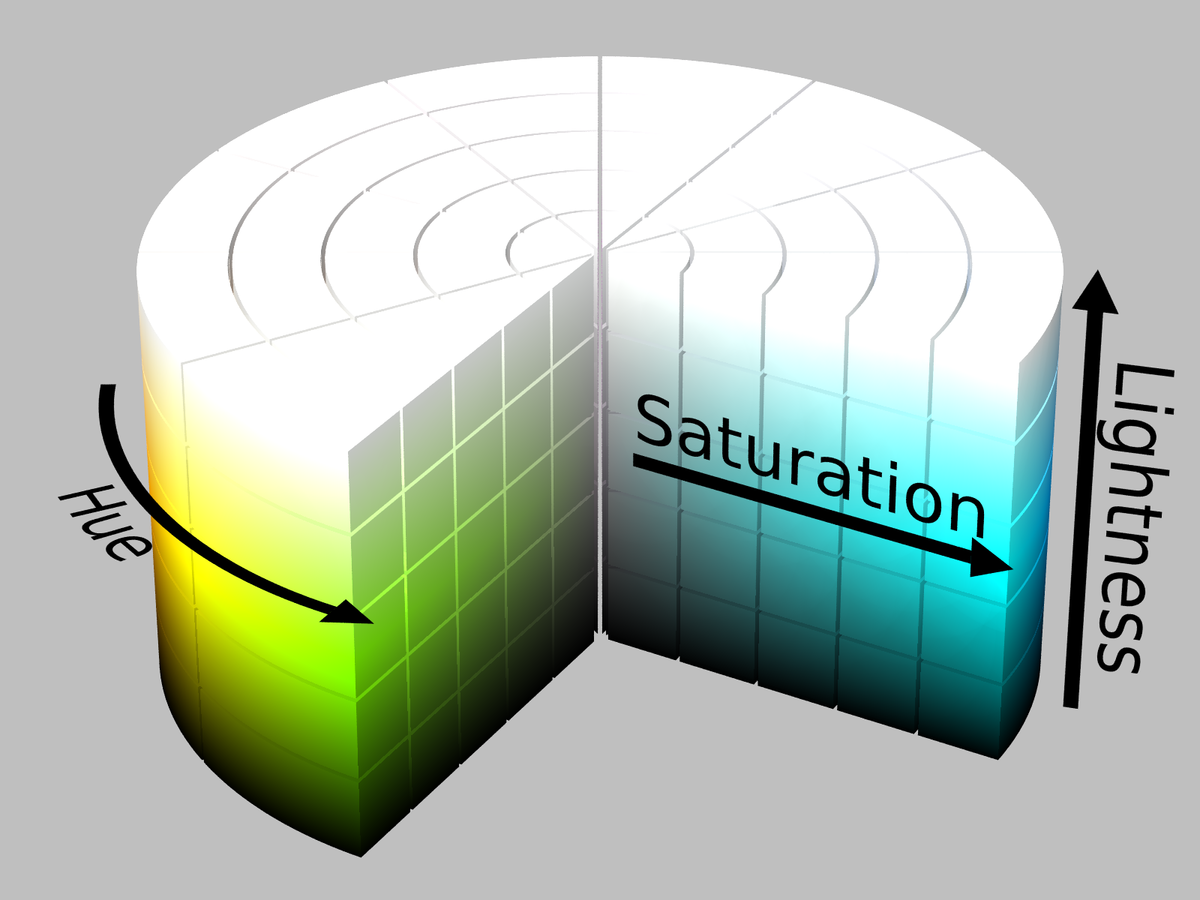
\includegraphics[width=0.48\textwidth]{Grafiken/HSL_Zylinder.png}
  \caption{Beispiel von Farbkörpern für HSV links und HSL rechts. Quelle: ~\cite{HSL_and_HSV_2023}}
  \label{fig:HSV_HSL}
\end{figure}

\paragraph{CIE 1931 XYZ}
Die CIE-Farbräume von 1931 sind die ersten definierten quantitativen Verbindungen zwischen den Verteilungen 
der Wellenlängen im elektromagnetischen sichtbaren Spektrum und den physiologisch wahrgenommenen Farben im menschlichen Farbsehen. 
Bei CIE XYZ werden die drei Farbkoordinaten X, Y und Z verwendet, um die Farbe zu beschreiben.
Dabei ist Y die Lumineszenz, Z ist ähnlich zu Blau im RGB Farbraum und X ist eine Mischung der drei CIE RGB Kurven.
Vorteil ist hier, dass bei einem konstanten Y Wert die XZ Fläche alle Farben dieser Lumineszenz enthält~\cite{CIE_1931_color_space_2023}.

\paragraph{CIELAB}
Der CIELAB Farbraum wurde 1976 von der CIE entwickelt.
CIELAB hat drei dinemsionen und erstreckt sich über den gesamten Gamut des menschlichen Farbsehens (siehe Grafik \ref{fig:CIELAB}).
Die drei Farbkoordinaten orientieren sich ebenfalls an der menschlichen Wahrnehmung, 
wo Rot und Grün, sowie Blau und Gelb als komplementäre Farben wahrgenommen werden.
Um dies aufzugreifen werden die Farbkoordinaten L, a und b verwendet.
Die L-Achse ist die Helligkeit und definiert 0 als Schwarz und 100 als Weiß.
Die a-Achse ist eine Relative Achse für die Farbtonkomplementarität von Rot und Grün.
Negative Werte gehen in Richtung Grün, positive Werte in Richtung Rot.
Die b-Achse ist eine Relative Achse für die Farbtonkomplementarität von Blau und Gelb.
Negative Werte gehen in Richtung Blau, positive Werte in Richtung Gelb.
CIELAB wird immer in relation zu einem Referenzweiß definiert, 
wofür CIE die Nutzung von CIE Standard illuminant D65 empfiehlt ~\cite{CIELAB_color_space_2023}.

\begin{figure}
  \centering
  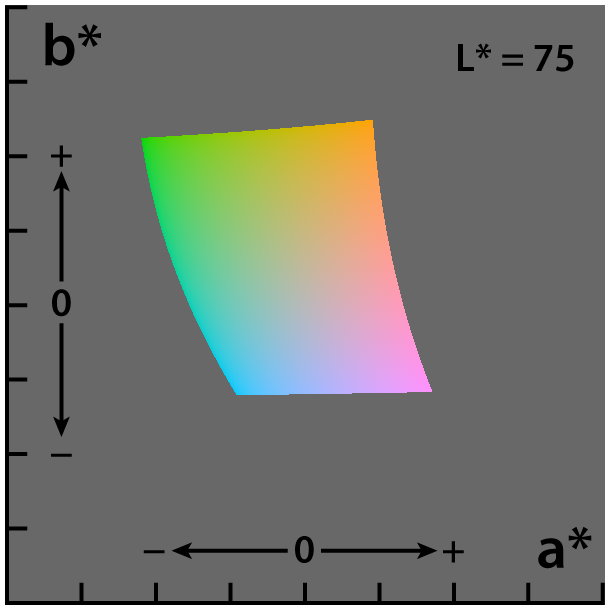
\includegraphics[width=0.29\textwidth]{Grafiken/CIELAB1.png}
  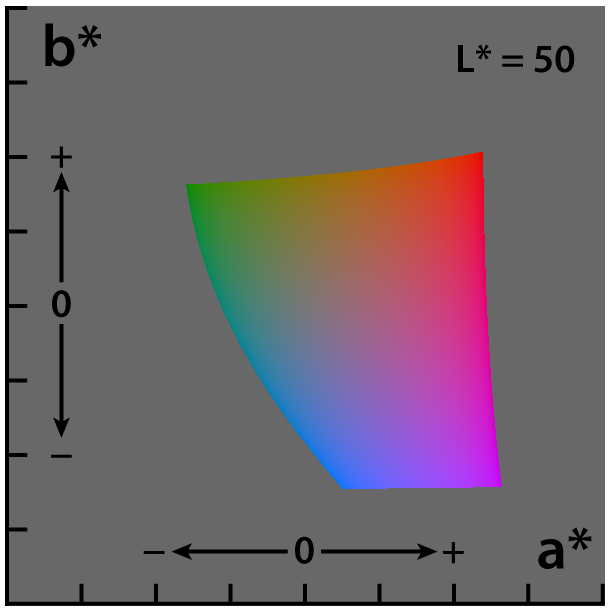
\includegraphics[width=0.29\textwidth]{Grafiken/CIELAB2.png}
  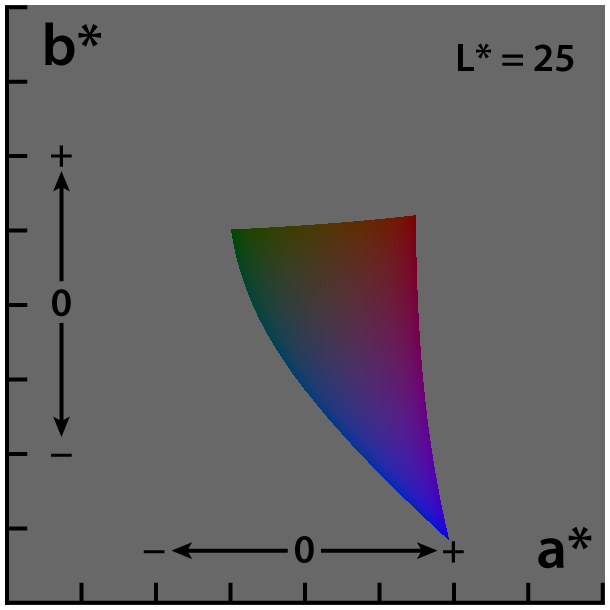
\includegraphics[width=0.29\textwidth]{Grafiken/CIELAB3.png}
  \caption{a*b* Farbebene des CIELAB Farbraumes bei unterschiedlichen L* Werten. Quelle: ~\cite{CIELAB_color_space_2023}}
  \label{fig:CIELAB}
\end{figure}

\paragraph{CAM16-UCS}
In der Farbmetrik ist der OSA-UCS (Optical Society of America Uniform Color Space) ein Farbraum, 
der erstmals 1947 veröffentlicht und vom Committee on Uniform Color Scales der Optical Society of America entwickelt wurde.
Der Ausschuss beschloss, dass eine neue Form verwendet werden muss, 
um einheitliche Farbunterschiede in jeder Richtung genau darstellen zu können.
Die drei dimensionen des Farbraumes sind sehr ähnlich zu CIELAB.
Die L-Achse ist die Helligkeit, die j-Achse ist die Farbtonkomplementarität von Blau und Gelb, 
wobei positive Werte gelber sind und negative Werte blauer sind.
Die g-Achse ist die Farbtonkomplementarität von Rot und Grün, 
wobei positive Werte grüner sind und negative Werte sind pinker ~\cite{OSA-UCS_2023}.

\paragraph{IPT}
Der IPT Farbraum ist ein dreidimensionaler Farbraum.
I steht für die Intensität und P und T ähneln a* und b* von CLAB. 
P beschreibt die Rot-Grün Dimension und T beschreibt die Blau-Gelb Dimension.
Die Vorteile von IPT sind, dass es eine bessere Repräsentation von hue 
in Anlehnung an die menschliche Wahrnehmung bietet. 
Außerdem ist IPT sehr simpel Konzipiert und lässt sich sehr einfach aus dem CIEXYZ Farbraum berechnen ~\cite{Ebner_1998}.

\section{Der Oklab Farbraum}
\subsection{Das Problem mit herkömmlichen Farbräumen}
\subsection{Motivation für Oklab}
\paragraph{Helmholtz-Kohlrausch Effekt}
\subsection{Herleitung von Oklab}
\subsection{Wie gut ist Oklab?}
\subsection{Bessere Sättigungskorrektur mittels Oklab}
% Von dem anderen Artikel
\subsection{Oklab in der Praxis}

% Bibliography
\printbibliography

\end{document}
